\ifspanish

\else

Consider the markov chain $X_k$ given by state space ${\cal S} = \{0,1,2,3\}$ and transition probability matrix
\[P = \begin{pmatrix}
      1-p & p & 0   & 0 \\
      0   & 0 & 1   & 0  \\
      0   & 0 & 1-p & p   \\
      0   & p & 0   & 1-p 
\end{pmatrix}\]
It is known that the initial state is $X_0=0$ with probability 1.

\begin{parts}
\part[5] Draw the transition graph.
\part[7] Compute the state probability distribution at time $k=2$. 
\part[8] Find the stationary distribution.
\part[5] Find the expected value of the time to reach state 1 for the first time.
\end{parts}


%%%%%%%%%%%%%%%%
\begin{solution}
\begin{parts}

\part The figure shows the transition graph for $p=0.2$:
\begin{center}
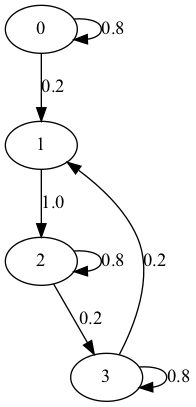
\includegraphics[width=0.15\textwidth]{./db/figs/mc_202405.png}
\end{center}

\part Since $X_0=0$, the initial state vector is \( q_0 = \begin{pmatrix} 1 & 0 & 0 & 0 \end{pmatrix}^\top \). Thus, the probability distribution at $k=2$ is
\begin{align*}
{\bf q}_2
	&= {\bf P}^\top {\bf P}^\top {\bf q}_0   \\
	&= \begin{pmatrix}
       1-p & p & 0   & 0 \\
       0   & 0 & 1   & 0  \\
       0   & 0 & 1-p & p   \\
       0   & p & 0   & 1-p 
      \end{pmatrix}^\top
      \cdot
	  \begin{pmatrix}
       1-p & p & 0   & 0 \\
       0   & 0 & 1   & 0  \\
       0   & 0 & 1-p & p   \\
       0   & p & 0   & 1-p 
      \end{pmatrix}^\top
      \cdot
	  \begin{pmatrix}
       1 \\ 0 \\ 0\\ 0 
      \end{pmatrix}   \\
	&= \begin{pmatrix}
       1-p & p & 0   & 0 \\
       0   & 0 & 1   & 0  \\
       0   & 0 & 1-p & p   \\
       0   & p & 0   & 1-p 
      \end{pmatrix}^\top
      \cdot
	  \begin{pmatrix}
       1-p \\ p \\ 0   \\ 0
      \end{pmatrix}
	 = \boxed{
	   \begin{pmatrix} (1-p)^2 \\ p (1-p) \\ p \\ 0 \end{pmatrix}
	   }
\end{align*}

\part The stationary distribution $\boldsymbol{\pi}$ is the solution of
\begin{align*}
\begin{pmatrix}
-p &  0 &  0 &  0 \\
 p  & -1 &  0 &  p  \\
 0  &  1 & -p &  0   \\
 0  &  0 &  p & -p \\
 1  &  1 &  1 &  1
\end{pmatrix} \cdot
\begin{pmatrix}  \pi_0 \\ \pi_1 \\ \pi_2 \\ \pi_3 \end{pmatrix}
= \begin{pmatrix} 0 \\ 0 \\ 0  \\ 1 \end{pmatrix}
\end{align*}

The first line shows that $\pi_0 = 0$. Taking it into account and removing the 4th equation, which is redundant, we get the simplified equation
\begin{align*}
\begin{pmatrix}
-1 &  0 & p  \\
 1 & -p & 0   \\
 1 &  1 & 1
\end{pmatrix} \cdot
\begin{pmatrix}  \pi_1 \\ \pi_2 \\ \pi_3 \end{pmatrix}
= \begin{pmatrix} 0 \\ 0  \\ 1 \end{pmatrix}
\end{align*}
whose solution is $\begin{pmatrix}  \pi_1 \\ \pi_2 \\ \pi_3 \end{pmatrix}
= \frac{1}{2+p} \begin{pmatrix} p \\ 1  \\ 1 \end{pmatrix}$. Therefore
\begin{align*}
\boxed{\boldsymbol{\pi} = \frac{1}{2+p} \begin{pmatrix} 0 \\ p \\ 1  \\ 1 \end{pmatrix}}
\end{align*}

\part Let $T$ be the time to reach state $1$ for the first time. Since, at time $k=1$, $X_k$ can be 0 or 1 only, we can write
\begin{align*}
\mathbb{E}\{T\} 
	&= \mathbb{E}\{T \mid X_1=1\} P\{X_1=1\} + \mathbb{E}\{T \mid X_1=0\} P\{X_1=0\}  \\
	&= 1 \cdot p + (1 + \mathbb{E}\{T\}) (1-p)
\end{align*}
therefore
\begin{align*}
\boxed{\mathbb{E}\{T\} = \frac1p}
\end{align*}
[An alternative path to the solution is
\begin{align*}
\mathbb{E}\{T\} 
	&= \sum_{k=0}^{\infty} k P\{T=k\}  
	 = p \sum_{k=0}^{\infty} k (1-p)^{k-1}    \\
	&= \frac{p}{1-p} \lim_{n\rightarrow \infty} \frac{1-p - (n+1)(1-p)^{n+1} + n (1-p)^{n+2}}{p^2}
	 = \frac{1}{p}
\end{align*}
].

\end{parts}

\end{solution}
  

\fi

